\documentclass{beamer}


\usepackage{amssymb,amsmath}
\usepackage{graphicx}
\usepackage{url}
\usepackage{color}
\usepackage{relsize}		% For \smaller
\usepackage{url}			% For \url
\usepackage{epstopdf}	% Included EPS files automatically converted to PDF to include with pdflatex
\usepackage{pagenote}[continuous,page]

%For MindMaps
% \usepackage{tikz}%
% \usetikzlibrary{mindmap,trees,arrows}%

%%% Color Definitions %%%%%%%%%%%%%%%%%%%%%%%%%%%%%%%%%%%%%%%%%%%%%%%%%%%%%%%%%
%\definecolor{bordercol}{RGB}{40,40,40}
%\definecolor{headercol1}{RGB}{186,215,230}
%\definecolor{headercol2}{RGB}{80,80,80}
%\definecolor{headerfontcol}{RGB}{0,0,0}
%\definecolor{boxcolor}{RGB}{186,215,230}

%%% Save space in lists. Use this after the opening of the list %%%%%%%%%%%%%%%%
%\newcommand{\compresslist}{
%	\setlength{\itemsep}{1pt}
%	\setlength{\parskip}{0pt}
%	\setlength{\parsep}{0pt}
%}

%\setbeameroption{show notes on top}

% You should run 'pdflatex' TWICE, because of TOC issues.

% Rename this file.  A common temptation for first-time slide makers
% is to name it something like ``my_talk.tex'' or
% ``john_doe_talk.tex'' or even ``discrete_math_seminar_talk.tex''.
% You really won't like any of these titles the second time you give a
% talk.  Try naming your tex file something more descriptive, like
% ``riemann_hypothesis_short_proof_talk.tex''.  Even better (in case
% you recycle 99% of a talk, but still want to change a little, and
% retain copies of each), how about
% ``riemann_hypothesis_short_proof_MIT-Colloquium.2000-01-01.tex''?

\mode<presentation>
{
  % A tip: pick a theme you like first, and THEN modify the color theme, and then add math content.
  % Warsaw is the theme selected by default in Beamer's installation sample files.

  %%%%%%%%%%%%%%%%%%%%%%%%%%%% THEME
  %\usetheme{Madrid}		% No subsection
  \usetheme{AnnArbor}  % Subsection on top, no color


  %\usetheme{Antibes}
  %\usetheme{Bergen}
  %\usetheme{Berkeley}		% bem bacana - menu esquerdo
  %\usetheme{Berlin}
  %\usetheme{Boadilla}
  %\usetheme{boxes}
  %\usetheme{CambridgeUS}		% bem bacana - menu superior
  %\usetheme{Copenhagen}
  %\usetheme{Darmstadt}
  %\usetheme{default}
  %\usetheme{Dresden}
  %\usetheme{Frankfurt}
  %\usetheme{Goettingen}
  %\usetheme{Hannover}		% bem bacana - menu esquerdo
  %\usetheme{Ilmenau}
  %\usetheme{JuanLesPins}
  %\usetheme{Luebeck}
  %\usetheme{Malmoe}
  %\usetheme{Marburg}		% bem bacana - menu direito
  %\usetheme{Montpellier}
  %\usetheme{PaloAlto}		% bem bacana - menu esquerdo
  %\usetheme{Pittsburgh}
  %\usetheme{Rochester}		%bacana
  %\usetheme{Singapore}
  %\usetheme{Szeged}
  %\usetheme{Warsaw}

  %%%%%%%%%%%%%%%%%%%%%%%%%%%% COLOR THEME
  %\usecolortheme{default}		% branco, azul clarinho
  \usecolortheme{crane}		% Very yellow (ok)

  %\usecolortheme{albatross}		% azul escuro, massa
  %\usecolortheme{beetle}		% cinza, menu azul
  %\usecolortheme{dolphin}		% azul e branco, legal
  %\usecolortheme{dove}			% cinza e branco, feio
  %\usecolortheme{fly}			% todo cinza, horrível
  %\usecolortheme{lily}			% parece o default
  %\usecolortheme{orchid}		% azul e branco, ok
  %\usecolortheme{rose}			% branco e violeta-claro, bonito
  %\usecolortheme{seagull}		% cinza, feio
  %\usecolortheme{seahorse}		% nhé, meio feio
  %\usecolortheme{sidebartab}		% Azul, branco, destaque na tab, interessante
  %\usecolortheme{structure}		% bichado
  %\usecolortheme{whale}		% Azul e branco, bem bonito

  %%%%%%%%%%%%%%%%%%%%%%%%%%%% OUTER THEME
  \useoutertheme{default}
  %\useoutertheme{infolines}
  %\useoutertheme{miniframes}
  %\useoutertheme{shadow}
  %\useoutertheme{sidebar}
  %\useoutertheme{smoothbars}
  %\useoutertheme{smoothtree}
  %\useoutertheme{split}
  %\useoutertheme{tree}

  %%%%%%%%%%%%%%%%%%%%%%%%%%%% INNER THEME
  \useinnertheme{circles}
  %\useinnertheme{default}
  %\useinnertheme{inmargin}
  %\useinnertheme{rectangles}
  %\useinnertheme{rounded}

  %%%%%%%%%%%%%%%%%%%%%%%%%%%%%%%%%%%

  \setbeamercovered{invisible} % or whatever (possibly just delete it)
  % To change behavior of \uncover from graying out to totally
  % invisible, can change \setbeamercovered to invisible instead of
  % transparent. apparently there are also 'dynamic' modes that make
  % the amount of graying depend on how long it'll take until the
  % thing is uncovered.

}


% Get rid of nav bar
\beamertemplatenavigationsymbolsempty

% Use short top
%\usepackage[headheight=12pt,footheight=12pt]{beamerthemeboxes}
%\addheadboxtemplate{\color{black}}{
%\hskip0.5cm
%\color{white}
%\insertshortauthor \ \ \ \
%\insertframenumber \ \ \ \ \ \ \
%\insertsection \ \ \ \ \ \ \ \ \ \ \ \ \ \ \ \ \  \insertsubsection
%\hskip0.5cm}
%\addheadboxtemplate{\color{black}}{
%\color{white}
%\ \ \ \
%\insertsection
%}
%\addheadboxtemplate{\color{black}}{
%\color{white}
%\ \ \ \
%\insertsubsection
%}

% Insert frame number at bottom of the page.
% \usefoottemplate{\hfil\tiny{\color{black!90}\insertframenumber}}

%% makes the ppagenote command for figure references at the end.

\usepackage[english]{babel}
%qq\usepackage[latin1]{inputenc}
\usepackage{CJKutf8}
\usepackage{subfigure}

\usepackage{times}
\usepackage[T1]{fontenc}

\makepagenote
\renewcommand{\notenumintext}[1]{}
\newcommand{\ppagenote}[1]{\pagenote[Page \insertframenumber]{#1}}

\title[Programming Challenges]{GB20602 - Programming Challenges}
\author[Claus Aranha]{Claus Aranha\\{\footnotesize caranha@cs.tsukuba.ac.jp}}
\institute[U. Tsukuba]{University of Tsukuba, Department of Computer Sciences}


\title[GB21802]{GB21802 - Programming Challenges}
\subtitle[]{Week 0 - Introduction}
\author[Claus Aranha]{Claus Aranha\\{\footnotesize caranha\@@cs.tsukuba.ac.jp}}
\institute{Department of Computer Science}
\date{2015/4/10\\{\smaller(last updated: \today)}}

\begin{document}

\section{Introduction}
\subsection{Course Outline}

\begin{frame}
\maketitle
\end{frame}

\begin{frame}
  \frametitle{What is this course about?}
  \begin{block}{Course Goal}
    Improve programming abilities and familiarity with algorithms and techniques.
  \end{block}
  \begin{block}{Course Method}
    Every week you have to solve many hard, difficult \structure{Programming Challenges}    
  \end{block}
  
  \bigskip
  
   In short: Learn by Practice!
\end{frame}

\begin{frame}
  \frametitle{Important Notice: Languages}
  
  This course uses both English and Japanese. This year we will try the following division:
      
  \begin{alertblock}{Japanese}
  \begin{itemize}
    \item Friday's Classes (Problem Review)
    \item Questions (Any classes)
    \item Mail Communication
  \end{itemize}
  \end{alertblock}
  
  \begin{block}{English}
  \begin{itemize}
    \item Monday Classes (Algorithm Review)
    \item Lecture Notes
  \end{itemize}
  \end{block}
  
  \begin{exampleblock}{Programming Language for Assignments}
    C, C++, Java and Pascal
  \end{exampleblock}
\end{frame}

\begin{frame}
  \frametitle{Important Notice 2: This document}

  This presentation is available online on the MANABA page: 

  \medskip

  \url{https://manaba.tsukuba.ac.jp/ct/course_427760}

  \medskip

  You can register to the course using the code:

  \medskip

  1962775


\end{frame}


\section{Course Outline}
\subsection{Course Structure}

\begin{frame}
    \frametitle{Outline}
    
    \begin{block}{Two classes per week}
        \begin{itemize}   
        \item Each week has a theme (see Manaba Syllabus)
        \item Monday Class: Theme Explanation (\structure{English})
        \item Friday Class: Problem Solving and Q\&A (\alert{Japanese})
        \end{itemize}
    \end{block}
    
    \begin{block}{Solving Problems}
        \begin{itemize}
        \item Every week there are four programming assignments;
        \item Assignments follow the weekly theme;
        \item Automatic Submission and Evaluation System;
        \item Deadline is Sunday 23:59
        \end{itemize}   
    \end{block}
\end{frame}
    
\begin{frame}
  \frametitle{Outline}
  \begin{center}
    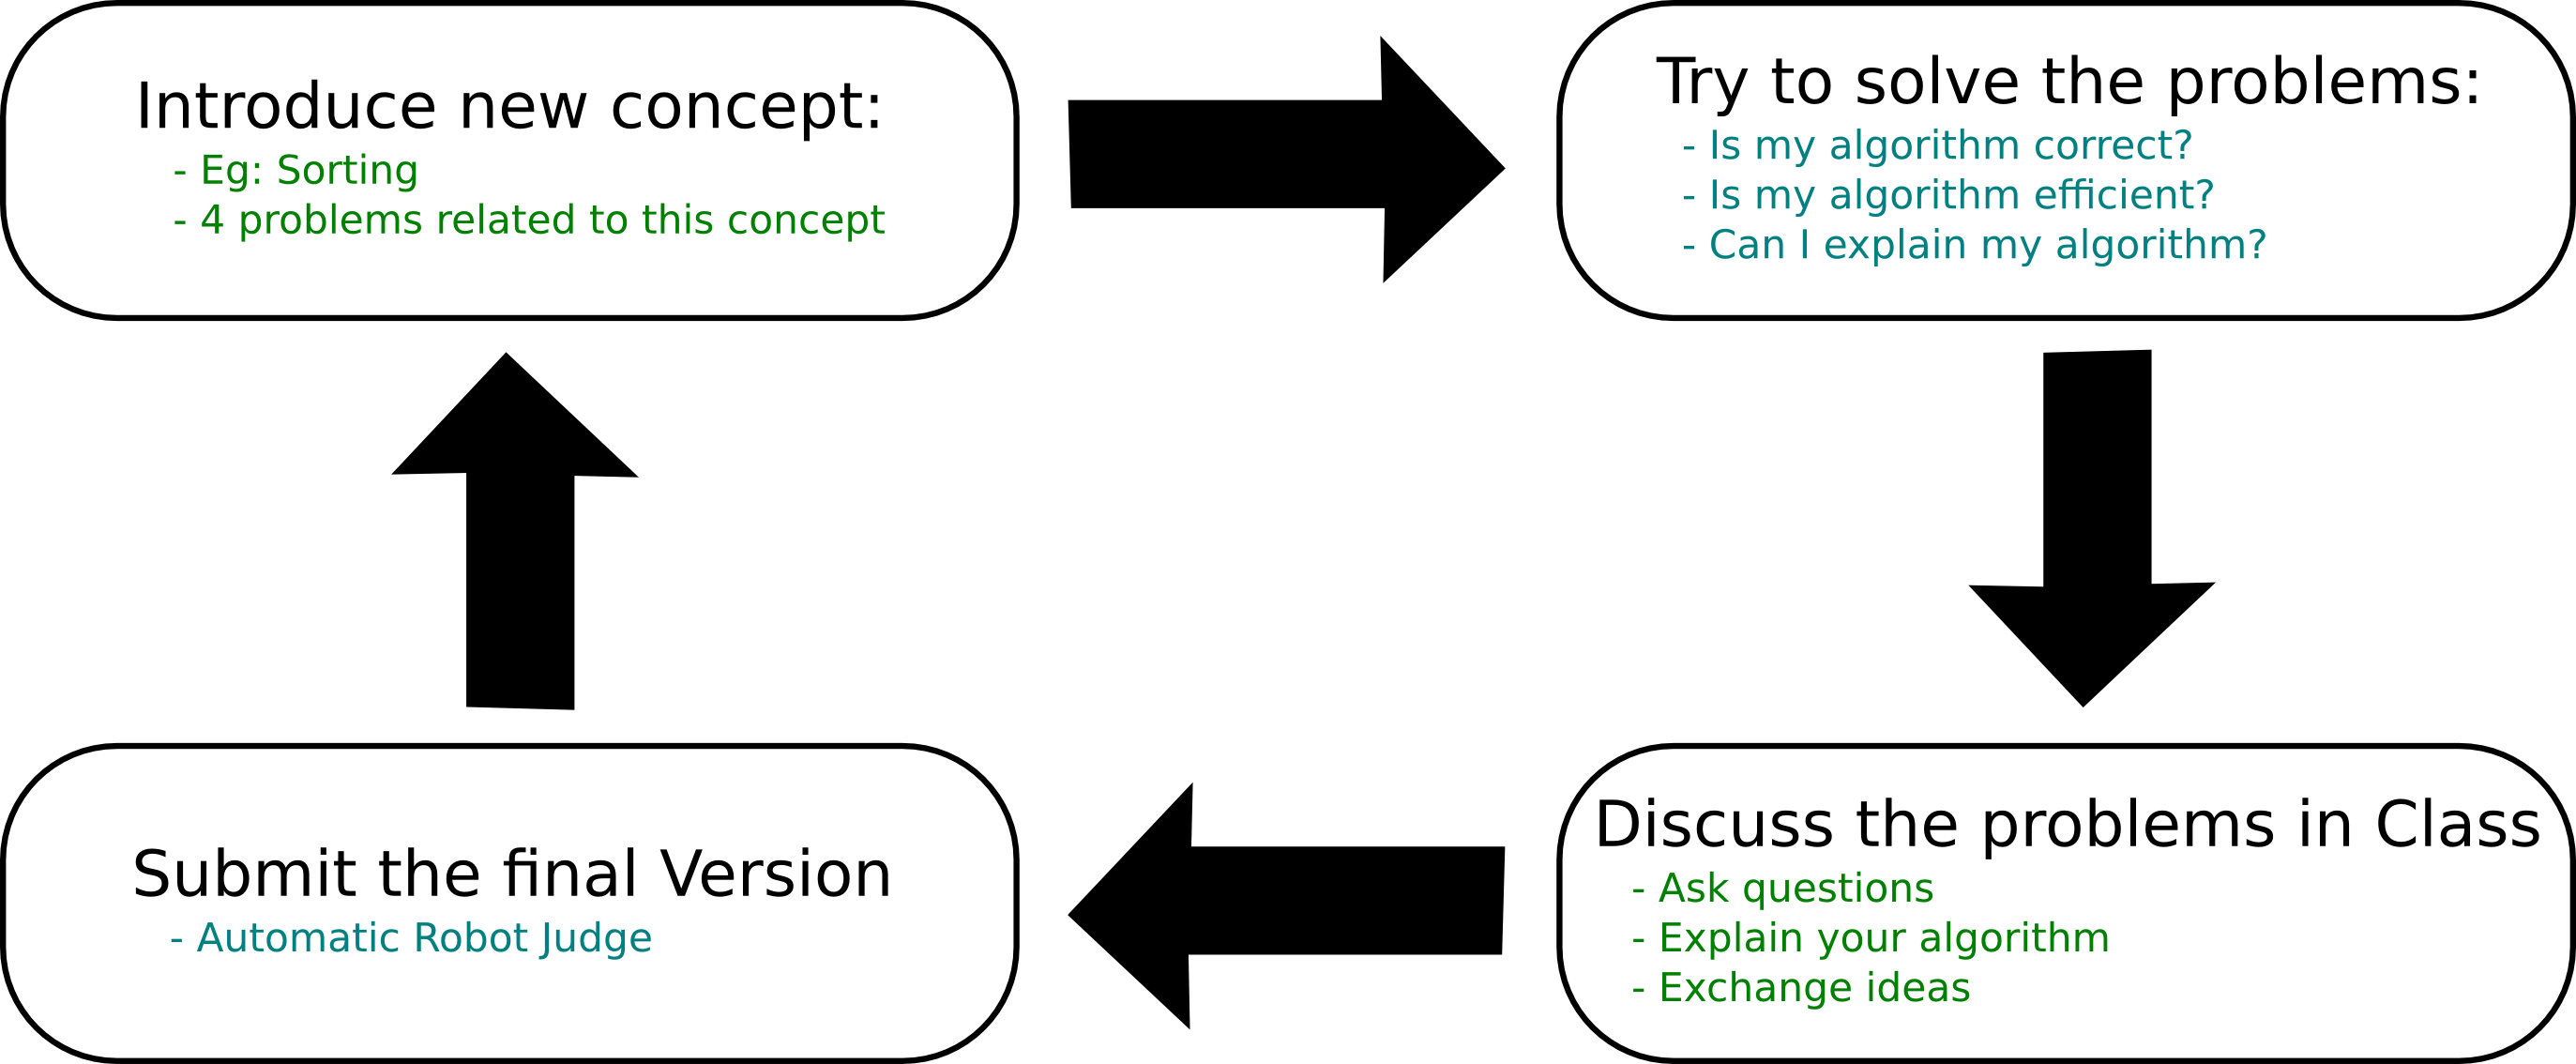
\includegraphics[width=1\textwidth]{classoutline}
  \end{center}
\end{frame}

\subsection{What is a Programming Challenge?}

% TODO: Break prog challenge description into pages
\begin{frame}
  \frametitle{What are programming challenges?}
  \begin{center}
    Short (but sometimes hard) problem involving algorithms
  \end{center}

  \begin{columns}[c]
    \column{0.35\textwidth}
    \begin{block}{Components}
      \begin{itemize}
      \item \alert<1>{Problem Outline}
      \item \alert<2-3>{Example Data}
      \item \alert<2-3>{Example Result}
      \item \alert<4>{Hidden Data}
      \item \alert<5>{Judge Result}
      \end{itemize}
    \end{block}
    \column{0.65\textwidth}
    \begin{block}{}
      \begin{onlyenv}<1>
        {\small
        Start with an integer n. If n is even, divide by 2. If n is
        odd, multiply by 3 and add 1. Repeat this process with the new
        value of n, terminating when n = 1. For example:\\
        \medskip
        22 11 34 17 52 26 13 40 20 10 5 16 8 4 2 1\\
        \medskip
        In the example above, the cycle length of 22 is 16. Given any
        two numbers i and j, you are to determine the maximum cycle
        length over all numbers between i and j, including both
        endpoints.}
      \end{onlyenv}
      \begin{onlyenv}<2>
        {\small
        {\bf Input}\\        
        The input will consist of a series of pairs of integers i and
        j, one pair of integers per line. All integers will be less
        than 1,000,000 and greater than 0.\\
        \smallskip

        {\bf Output}\\
        For each pair of input integers i and j, output i, j in the
        same order in which they appeared in the input and then the
        maximum cycle length for integers between and including i and
        j.}
      \end{onlyenv}
      \begin{onlyenv}<3-4>
        {\small
        {\bf Sample Input}\\
        1 10\\
        100 200\\
        201 210\\
        900 1000\\
        
        {\bf Sample Output}\\
        1 10 20\\
        100 200 125\\
        201 210 89\\
        900 1000 174\\}
      \end{onlyenv}
      \begin{onlyenv}<5>
        Accepted\\
        Rejected\\
        Time Limited Exceeded (TLE)\\
      \end{onlyenv}
    \end{block}
  \end{columns}
\end{frame}

\subsection{Grading}

\begin{frame}
  \frametitle{Evaluation and Grading (1)}

  Evaluation Criteria: \structure{Problems solved} and \structure{Participation}
  
  \begin{block}{Evaluation Base}
  \begin{itemize}
  \item \structure{C}: One problem per class;
  \item \structure{B}: Two problems per class,\\
    or One problem per class and 21 problems total;
  \item \structure{A}: Three problems per class,\\
    or One problem per class and 30 problems total;
  \end{itemize}
  \end{block}
\end{frame}

\begin{frame}
  \frametitle{Evaluation and Grading (2)}
  
  A \structure{Bonus} or \structure{Penalty} will be added to the base grade.
  \begin{itemize}
    \item Bonus: Change grade one step up (C->B, A->A+)
    \item Penalty: Change grade one step down (A+->A, B->C, \alert{C->C})
  \end{itemize}
  
  \medskip
  \begin{exampleblock}{Bonus: Grade Up}
    Good participation in class and good Comments in code.
  \end{exampleblock}
  \begin{alertblock}{Penalty: Grade Down}
    More than \alert{8} late problems.
  \end{alertblock}
\end{frame}

\section{Assignment System}
\subsection{How to submit problems}
\begin{frame}
  \frametitle{How to submit problems -- 1}

  Problem submission and evaluation will be done throught the

  \medskip

  \emph{Programming Challenges} website.
  \begin{center}
    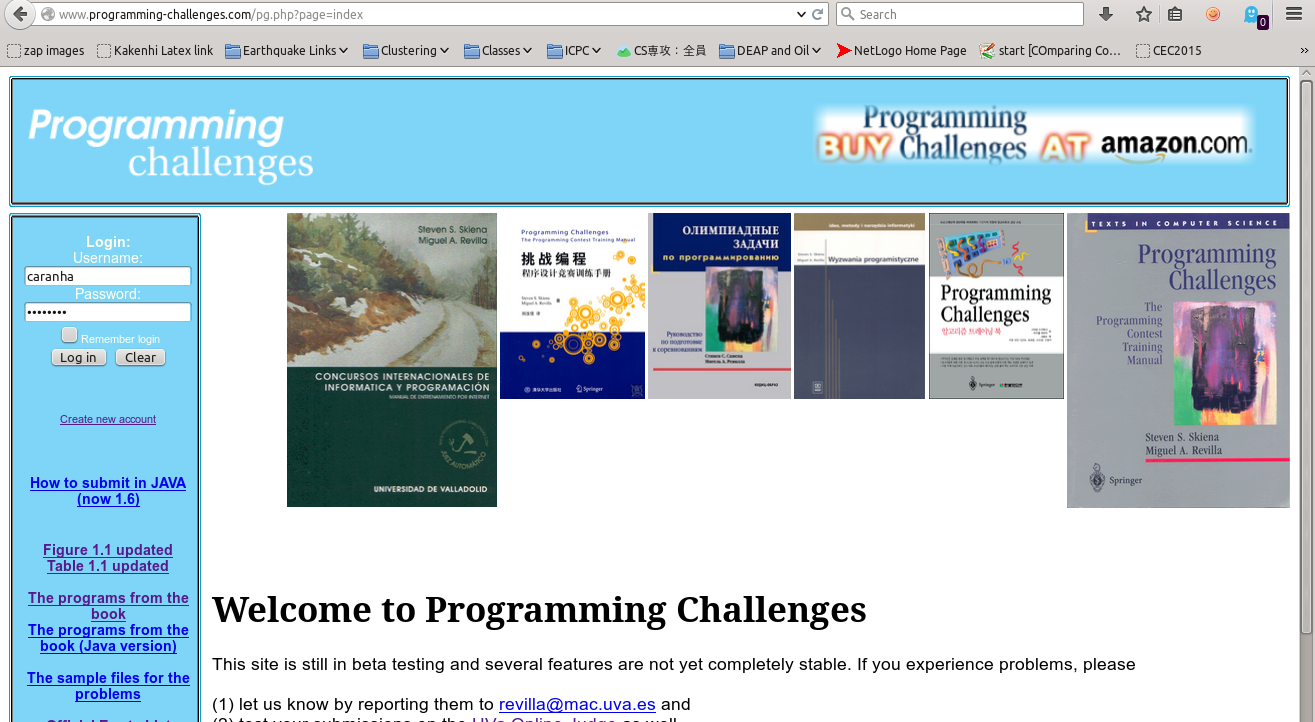
\includegraphics[height=0.4\textheight]{pcwebsite}
  \end{center}

  \medskip

  Access it at \url{http://www.programming-challenges.com/}
\end{frame}

\begin{frame}
  \frametitle{How to submit problems -- 2}
  \begin{enumerate}
      \item Make an account at \url{http://www.programming-challenges.com};\\ 
      \item Send your ID to me:
        \begin{itemize}
        \item Manaba Form\\
          or
        \item e-mail (caranha@cs.tsukuba.ac.jp)\\
          send your student number, name and ID
        \end{itemize}
      \item You will be added to the classroom\\
        \structure{Tsukuba~Programming~Challenges~2015}; 
  \end{enumerate}
\end{frame}


\begin{frame}
  \frametitle{How to submit problems -- 3}

  \begin{center}
    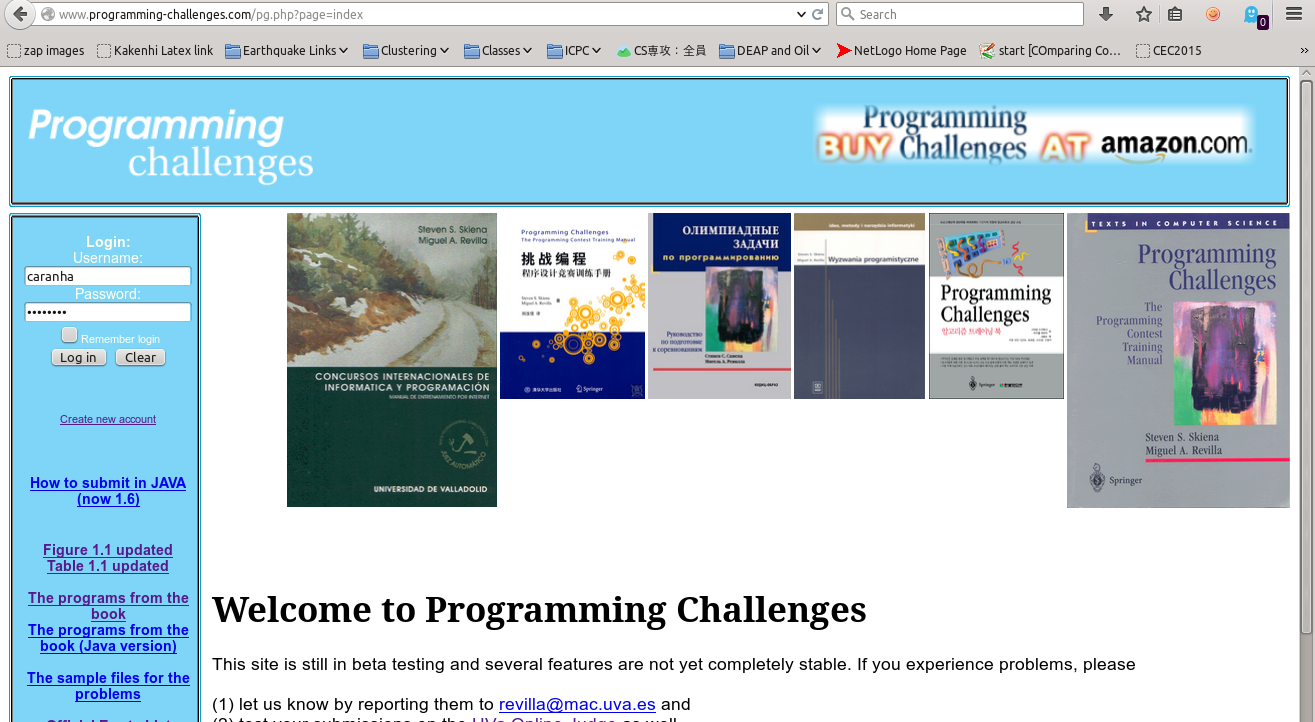
\includegraphics[height=0.4\textheight]{pcwebsite}
  \end{center}

  \begin{enumerate}
    \setcounter{enumi}{3}
  \item Click ``Joined Classrooms'', select
    \structure{Tsukuba~Programming~Challenges~2015};
  \item Click the name of the problem for a description, then ``Submit'' to send your code.
  \item Choose the language; upload a file or paste your code.
  \end{enumerate}
\end{frame}

\begin{frame}[simple,fragile]
  \frametitle{How to submit problems -- 4}

  Some notes about writing programs:
  
  \begin{block}{Input and Output}
    Input comes from the \structure{STDIN}, output comes from the \structure{STDOUT}.
  \end{block}

  \begin{exampleblock}{Good Comment}
    {\smaller
\begin{verbatim}
/**
 * I used quicksort to solve this problem. 
 * I sorted the age of the persons in the input.
 * To make it faster, people with the same age were 
 * removed from the data.
 */
\end{verbatim}}
  \end{exampleblock}
  \begin{alertblock}{Bad Comment}
{\smaller
\begin{verbatim}
/**
 * Quicksort.
 */
\end{verbatim}}
  \end{alertblock}
\end{frame}

\begin{frame}
  \frametitle{How to submit problems -- 5}
  \begin{block}{A warning about Java}
    \begin{itemize}
    \item Very high number of runtime problems -- beware!
      \medskip

    \item Main class MUST be named ``Main''
      \medskip

    \item Read the example code at:\\
      \url{http://www.programming-challenges.com/pg.php?page=javainfo}
    \end{itemize}
  \end{block}
\end{frame}

\subsection{Judge Evaluation}

\begin{frame}
  \frametitle{How the Judge Works}
  \begin{block}{Accepted}
    Congratulations!
  \end{block}
  \begin{block}{\alert{Wrong Answer}}
    \begin{itemize}
    \item Is your answer EXACTLY the same as expected?
    \item Check worst-case scenarios!
    \end{itemize}
  \end{block}
  \begin{block}{\alert{Time Limited Exceeded}}
    You need a more efficient algorithm.
  \end{block}
  \begin{block}{Compilation Error, Runtime Error}
    Check your Code!
  \end{block}
  % Accepted, Rejected, TLE, Presentation Error
\end{frame}

\begin{frame}
  \frametitle{Very Important!}
  
  The assignments are \alert{individual}. Use your own strength to solve the programs.

  \medskip
  
  \begin{itemize}
  \item Do not copy solutions from the internet;
  \item Do not copy solutions from your friends;
  
  \medskip
  
  \item It is okay to use for \underline{ideas} from others or online;
  \item If you use an idea from someone else, \alert{make sure to give proper attribution} in the program comments
  \end{itemize}
  
  \begin{block}{}
    Plagiarism leads to course failure
  \end{block}
\end{frame}

\section{Resources}
\subsection{Resources}

\begin{frame}
    \frametitle{Useful Links}
    \begin{itemize}
        \item {\bf Manaba: } 
        {\smaller \url{https://manaba.tsukuba.ac.jp/ct/course_427760}}\\
        Manaba Code: 1962775

        \item {\bf Lecture Notes: } 
        {\smaller \url{https://github.com/caranha/ProgrammingChallengesLectureNotes}}\\
        Feel free to fork/pull!
        
        \item {\bf Professor Page: } 
        {\smaller \url{http://conclave.cs.tsukuba.ac.jp/?page_id=128}}\\
        Lecture notes and Announcements (please use manaba)
        
        \item {\bf Submission System: } 
        {\smaller \url{http://www.programming-challenges.com/pg.php?page=showclassroom&classid=1474}}
    \end{itemize}
\end{frame}

% TODO: Add information about books
\begin{frame}
    \frametitle{Reference Books}
    \begin{itemize}
        \item "Programming Challenges", Steven S. Skiena, Miguel A. Revilla
        \item "Competitive Programming"
        \item "Ant Book"
    \end{itemize}

    (I will add more information in manaba page later)

\end{frame}

\begin{frame}
    \frametitle{Contact Information}
    \begin{itemize}
    \item {\bf E-mail:} caranha@cs.tsukuba.ac.jp
    \item {\bf twitter:} caranha
    \end{itemize}

    \bigskip
    
    Feel free to contact me in English or Japanese!    
\end{frame}

\end{document}
